\section{选题的背景和意义}

模型检测(Model Checking)是一种自动化形式方法,用于验证有限状态系统的性质。模型检测最初由 E. M. Clarke 和 E. A. Emerson 提出\citep{Emerson_1980,Clarke,Clarke_1986},如今已广泛应用于软件和硬件设计。例如,在嵌入式系统中,可以使用 UML 活动图来验证硬件是否符合规范\citep{Grobelna_2015}。

模型检测将待检测的系统建模为一个跃迁系统(transition system),在时序逻辑(temporal logic)中指定待验证的属性。给定模型\(M\) 和属性\(\varphi\),模型检测将验证是否\(M\)满足\(\varphi\)。在不同的模型检测方法中,高级符号模型检查(Advanced Symbolic Model Checking)\citep{Grobelna_2015}使用简化的有序二叉决策图(Reduced Ordered Binary Decision Diagrams,ROBDDs 或 BDDs)\citep{Bryant_1986}来表示状态集合和转移关系。通过迭代调用图像计算算法来计算所有可达状态,判断一个模型是否满足时间属性,直到达到不动点为止。

最近,随着量子计算的发展,关于量子线路的验证技术也在不断发展\citep{viamontes2007checking,burgholzer2020advanced}。其中,利用模型检测方法对线路进行自动化验证也有了一些应用。由于量子线路运算空间随着量子比特的线性增加而指数级膨胀,传统的计算方法并不能很好应对。因此本次研究希望应用基于张量网络(tensor network)的张量决策图(tensor decision diagrams)进行量子模型检测。 
\subsection{量子计算简介}
量子计算机(quantum computer)是一种利用量子比特特性进行计算的一种设备。在量子计算中,量子比特的特殊性质允许其同时处于多种状态,这与经典比特的二进制状态不同。量子计算机的状态空间可以用希尔伯特空间(Hilbert space)\(\mathcal{H}\)表示\citep{nielsen2010quantum},即可以进行内积运算(inner product)的复向量空间。比特状态可以用\(\mathcal{H}\)的向量表示,量子门由\(\mathcal{H}\)上的酉算子(unitary operator)表示。

量子线路(quantum circuit)是一种描述量子计算的模型。在量子线路中,通过量子比特的初始化、应用量子门、测量以及其他可能的操作的序列来构建和执行量子计算任务。量子线路通常从左向右阅读,每个量子门的作用是将输入的量子比特状态转变为输出状态,该过程可以认为是量子门的酉矩阵与输入的量子状态的乘积。
\begin{figure}[!htbp]
    \centering
    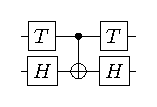
\includegraphics[width=.6\textwidth]{Img/example_cir.pdf}
    \caption{一个量子线路的例子}
    \label{fig:example_cir}
\end{figure}

图\ref{fig:example_cir} 所示的量子线路展示了一个具体的量子线路示例。其中有单比特门\(H=\frac{1}{\sqrt2}\left[\begin{matrix}1&1\\1&-1\\\end{matrix}\right],T=\left[\begin{matrix}1&0\\0&e^{-i\pi/4}\\\end{matrix}\right]\),以及双比特门\(CX=\left[\begin{matrix}\begin{matrix}1&0\\0&1\\\end{matrix}&\begin{matrix}0&0\\0&0\\\end{matrix}\\\begin{matrix}0&0\\0&0\\\end{matrix}&\begin{matrix}0&1\\1&0\\\end{matrix}\\\end{matrix}\right]\)。假设该量子线路的初始状态为\(\left|\psi\right\rangle=\left|\psi_1\right\rangle\left|\psi_2\right\rangle\),则输出状态为\(T\otimes H\cdot CX\cdot T\otimes H\cdot\left|\psi\right\rangle\)。

在量子计算机上可以执行各种算法和计算任务,如量子搜索\citep{Grover_1996}、量子因子分解\citep{shor}和量子模拟\citep{Feynman}等。量子计算的潜力在于其能够在某些特定问题上比经典计算机更高效地进行计算,尤其在处理大规模数据和解决复杂问题方面具有潜在优势。需要对这部分深入了解的读者,可以自行阅读\citep{nielsen2010quantum}。
\subsection{量子计算中的模型检验}
\subsubsection{跃迁系统}
跃迁系统广泛应用于模型检测中待检测系统的建模,其定义为\citep{baier2008principles}:
\begin{equation}
\mathcal{M}=\{S,Act,\rightarrow,I\}
\end{equation}
其中\(S\)为系统状态集合,\(I\)为系统初态集合,因此满足\(I\subseteq S\)。\(Act\)为系统行为集合。\(\rightarrow\)为系统状态转移关系,即\(\rightarrow\subset S\times Act\times S\)。此外还有\(AP\)为描述系统原子命题。L是标记函数,将状态映射为状态满足的原子命题集合。需要验证的属性\(\varphi\)将表述为命题。


系统的有限路径片段\(\pi\)是一个有限状态序列\(s_0,s_1\ldots s_n\)。\(s_i\)满足\(s_{i-1}\overset{a}{\rightarrow}s_i,a\in Act\),对于所有\(0<i\leq n\),其中\(n\geq 0 \)。无限路径片段\(\pi\)是一个无限状态序列\(s_0,s_1\ldots\),使得对于所有\(i>0\),\(s_{i-1} \overset{a}{\rightarrow}  s_i,a\in Act\)。在路径中\(\pi\left[i\right]=s_i,\pi\left[i\right)=s_i\ldots\)。所有以\(s_0\)为开始的路径,构成了路径集合\(Path\left(s_0\right)\)。

\begin{figure}[!htbp]
    \centering
    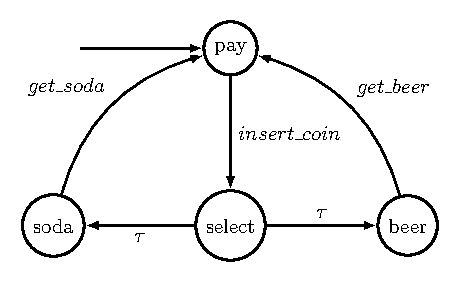
\includegraphics[width=.6\textwidth]{Img/map.pdf}
    \caption{一种简化版的售货机跃迁系统}
    \label{fig:transition-system}
\end{figure}

图\ref{fig:transition-system} 所示的跃迁系统展示了一个简化版的售货机模型。在该模型中,用户投入硬币,进行选择后就可以得到苏打水或者啤酒。在该例子中,系统状态\(S=\{pay,select,soda,beer\}\),系统初态\(I=pay\)。
系统行为\(Act=\{insert\_coin,\tau,get\_soda,get\_beer\}\),其中\(\tau\)表示立即行动符号。转移关系图中已经展示。原子命题可取\(AP=\{paid,drink\}\)。因此\(L\left( pay \right)=\{\varnothing\}\),\(L\left(soda\right)=L\left(beer\right)=\{paid,drink\}\),\(L\left(select\right)=\{paid\}\)。系统的一个路径是\(\pi=pay\ select\ soda\ pay\ selsect\ \ldots\)。此时\(\pi\left[1\right]=slect,\pi\left[1\right)=select\quad soda\quad pay\quad selsect\ldots\)。同时该路径满足\(\pi\in Path\left(pay\right)\)。
量子模型检测的跃迁系统类似。区别在于状态空间用\(\mathcal{H}\),转移关系用酉矩阵。一个量子自动机定义如下:
\begin{align}
    \mathcal{M}=\{\mathcal{H},Act,\{U_\alpha,\alpha\in Act\},\mathcal{H}_0\}
\end{align}
由于目前量子模型检测的发展还比较初期,因此需要验证的属性\(\varphi\)会表示为\(\mathcal{H}\)的一个子空间。
\subsubsection{时序逻辑}
在量子模型检测中,与经典模型检测一样使用时序逻辑指定待验证的属性\(\varphi\)。时序逻辑命题的运算符有两类\citep{goranko_2023}。状态命题公式(State formulas):\(\varphi ::=a\left|\exists\varphi\right|\forall \varphi\left|\lnot\varphi\right|\varphi\land\psi\),其中\(a\in AP\)。以及路径命题公式(Path formulas):\(\varphi\Colon=O\varphi|\varphi U\psi\)。给定模型的一个状态为\(s\),路径为\(\pi\),则具体满足条件分别如下:
\begin{itemize}
    \item \(s\models a,iff \L\left(s\right)\models a\)
    \item \(s\models\exists\varphi,iff\ \pi\models\varphi\)对一些\(\pi\in Path\left(s\right)\)
    \item \(s\models\forall\varphi,iff\ \pi\models\varphi\)对所有\(π\in Paths\)
    \item \(s\models\lnot\varphi,iff\ s\nvDash\varphi\)
    \item \(s\models\varphi\land\psi,iff\ s\models\varphi\ and\ s\models\psi\)
    \item \(\pi\models O\varphi,iff\ \pi\left[1\right]\models\varphi\)
    \item \(\pi\models\varphi U\psi,iff\ \exists j\geq0\).\(\pi\left[j\right)\models\psi\) 同时对所有\(0\le i<j\)有\(\pi\left[i\right)\models\varphi\)
\end{itemize}


图\ref{fig:path-formula-basic} 展示了两种路径命题公式的直观示意图。


\begin{figure}[!htbp]
    \centering
    \begin{subfigure}[b]{0.8\textwidth}
        \centering
        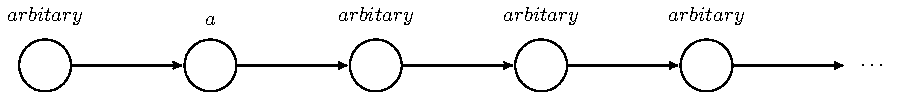
\includegraphics[width=\textwidth]{Img/path_for_Oa.pdf}
    \end{subfigure}
    \\
    \begin{subfigure}{0.8\textwidth}
        \centering
        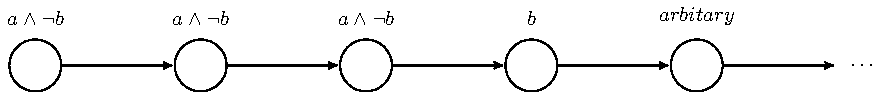
\includegraphics[width=\textwidth]{Img/path_for_aUb.pdf}
    \end{subfigure}
    \caption{$\pi\models O a $与 $\pi\models a U b$的图示}
    \label{fig:path-formula-basic}
\end{figure}
\subsubsection{可达性问题}
在模型检测中,有三类比较重要的可达性问题,分别是可达性、持续可达性以及重复可达性。本次研究内容就是设计基于TDD的量子模型检测,从而对给定的模型和属性,计算对应的可达概率。过程中主要涉及以下路径命题公式:\(\lozenge\) 表示最终(eventually),\(\square\)表示总是(always),\(\lozenge\square\)表示总是最终(always eventually),\(\square\lozenge\)表示最终总是(eventually always)。其中\(\lozenge\)和\(\square\)具体定义为:
\begin{itemize}
    \item \(\lozenge\varphi\overset{\text{def} }{=} \text{True}U\varphi\)
    \item \(\square\varphi\overset{\text{def} }{=} \neg\lozenge\neg\varphi\)
\end{itemize}
图\ref{fig:path-formula}展示了这两种基本路径命题公式的直观示意图。
\begin{figure}[!htbp]
    \centering
    \begin{subfigure}[b]{0.8\textwidth}
        \centering
        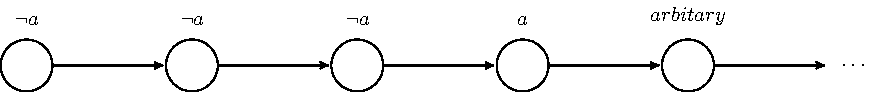
\includegraphics[width=\textwidth]{Img/path_for_Dia.pdf}
    \end{subfigure}
    \\
    \begin{subfigure}{0.8\textwidth}
        \centering
        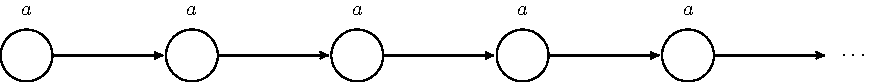
\includegraphics[width=\textwidth]{Img/path_for_SQa.pdf}
    \end{subfigure}
    \caption{$\pi\models\lozenge a$与 $\pi\models\square a$的图示}
    \label{fig:path-formula}
\end{figure}

具体的可满足条件为:
\begin{itemize}
    \item \(\pi\models\lozenge\varphi,iff\exists j\ge0.\pi[j)\models\varphi\)
    \item \(\pi\models\square\varphi,iff\forall j\ge 0.\pi[j)\models\varphi\)
    \item \(\pi\models\lozenge\square\varphi,iff\exists i\ge 0.\forall j\ge i,\pi[j)\models\varphi\)
    \item \(\pi\models\square\lozenge\varphi,iff\forall i\ge 0.\exists j\ge i,\pi[j)\models\varphi\)
\end{itemize}
基于此三种可达性问题定义分别如下:
\begin{itemize}
    \item 可达性:\( Pr^{\mathcal{M}}(s \models \lozenge G) = Pr^M(\pi \models \lozenge G : \pi \in \text{Paths}(s))\)
    \item 持续可达性:\( Pr^{\mathcal{M}}(s \models \lozenge \square G) = Pr^M(\pi \models \lozenge \square G : \pi \in \text{Paths}(s))\)
    \item 重复可达性:\( Pr^{\mathcal{M}}(s \models\square \lozenge G) = Pr^M(\pi \models \square\lozenge G : \pi \in \text{Paths}(s))\)
\end{itemize}
	
对于量子模型检测的可达性问题的解决,一种直接的解决办法是计算路径上每个状态,然后与待检测属性比较。但是量子计算中状态空间\(\mathcal{H}\)维度\(dim\left(\mathcal{H}\right)=2^n\),其中n为比特数量。即状态空间维数随比特个数指数级增长。因此需要使用新的数据结构,以降低复杂度。
\subsection{Tensor Decision Diagrams(TDD)}
\subsubsection{张量网络表示量子线路}
张量是与一组与索引\(I=\{x_1,\ldots,x_n\}\)相关联的多维线性映射。在量子计算中,可以假设只从\(\{0,1\}\)中取值。因此,张量定义为:
\begin{align}
    \phi :{\{0,1\}}^I\rightarrow\mathbb{C}
\end{align}
其中\(\mathbb{C}\)为实数。张量网络是一个无向图\(G=\left(V,E\right)\)。其中顶点集V中的每个顶点v表示一个张量。边集\(E\)中每条边\(e\)代表与相邻两个张量相关联的公共索引。通过以任意顺序收缩连接的张量,可以得到一个秩为\(m\)的张量,其中\(m\)是$G$中开放边数。这个独立于收缩顺序的张量也称为该张量网络的张量表示\citep{biamonte2019lectures}。
张量网络提供了一种新的量子线路表示方法\citep{pednault2017breaking}。一个向量表示为$[\alpha_0,\alpha_1]$的量子比特x可以描述为秩为1的张量$\phi_x$,其中$\phi_x\left(0\right)=\alpha_0, \phi_x\left(1\right)=\alpha_1$。具有输入比特x和输出比特y的单比特门可以表示为秩2张量$\phi_{xy}$。例如,以x作为输入比特和y作为输出比特的单比特门Z-gate的张量表示:$\phi_{xy}\left(00\right)=1,\phi_{xy}\left(01\right)=\phi_{xy}\left(10\right)=0,\phi_{xy}\left(11\right)=-1$。类似的$n$比特量子门可以表示成一个秩为$2n$的张量。在张量表示中,一般不区分输入和输出索引。只有当将张量解释为门或电路时会规定关于其信息。

给定量子线路中所有量子门的输入和输出状态的索引值,就可以得到量子电路的张量表示。图\ref{fig:example_cir_map}给定了图\ref{fig:example_cir}中量子线路中各个状态的索引值,从而可得的张量表示:
\begin{align}
\phi_{x_0x_3y_0y_3}\left(a_0a_3b_0b_3\right)=\sum_{a_1,a_2,b_1,b_2=0}^{1}T\left(a_0a_1\right)H\left(b_0b_1\right)CX\left(a_1b_1a_2b_2\right)T\left(a_2a_3\right)H\left(b_2b_3\right)
\end{align}

\begin{figure}[!htbp]
    \centering
    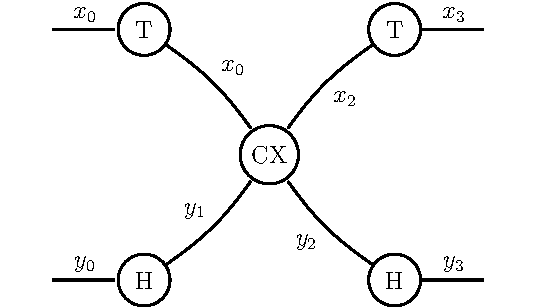
\includegraphics[width=.6\textwidth]{Img/tensor_example.pdf}
    \caption{用张量表示图\ref{fig:example_cir}中量子线路}   
    \label{fig:example_cir_map}
\end{figure}

\subsubsection{张量决策图}
张量决策图(Tensor Decision Diagrams,或TDD)是一种具有决策图和张量网络特征的数据结构\citep{Hong_2022}。它可用于表示张量和量子电路。与BDD(Boolean Decision Diagrams)类似,TDD是一种建立在索引顺序$I=\{x_1,\ldots,x_n\}$上的决策树模型。具体定义如下:
\begin{align}
    \mathcal{F}=\left(V,E,index,value,low,high,w\right)
\end{align}
其中$V$是一个有限节点集,被划分为非终端节点$V_n$和终端节点$V_T$。用$r_{\mathcal{F}}$表示$\mathcal{F}$的唯一根节点。$E=\left\{\left(v,low\left(v\right)\right),\left(v,high\left(v\right)\right):v\in V_N\right\}$是树中所有边集合,其中$\left(v,low\left(v\right)\right)$和$\left(v,high\left(v\right)\right)$分别称为v的低边和高边。根结点$r_{\mathcal{F}}$具有唯一的入射边$e_{\mathcal{F}}$,该入射边没有源结点。$index:V_r\rightarrow I$将每个非终端节点分配给I中的索引。$value:V_T\rightarrow\mathbb{C}$将每个终端节点赋予一个复数值。$low$和$high$都是$V_N\rightarrow V$中的映射,它们分别为每个非终端节点指定其低边和高边后继。$w:E\rightarrow\mathbb{C}$将每条边赋予一个复数权重。特别地,$w\left(e_r\right)$称为$\mathcal{F}$的权重,并记作$w_{\mathcal{F}}$。 



图\ref{fig:tdd_ex} 展示了一个TDD的例子。其中索引顺序$I=\{x_0,y_0,y_3\}$。非终端节点$V_n$用圆表示,终端节点$V_T$用方形表示。每个节点的低边用虚线表示,高边用实线表示。该示例中各边的权重均为1,即$w:E\rightarrow 1$。根节点$r_{\mathcal{F}}=x_0$。决策树的权重$w_{\mathcal{F}}=1$。
\begin{figure}[!htbp]
    \centering
    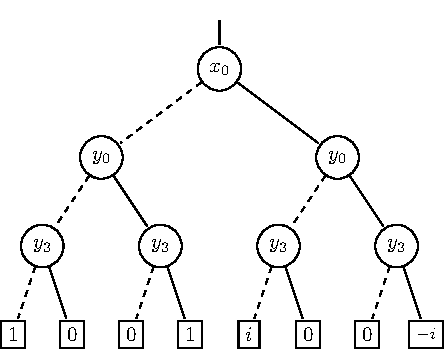
\includegraphics[width=.6\textwidth]{Img/tree_tdd.pdf}
    \caption{一个TDD示例}   
    \label{fig:tdd_ex}
\end{figure}

对于TDD中的一个节点$v$,如果$v$是终端节点,则$\phi\left(v\right):= valuev$是一个秩为$0$的张量,即常数。如果$v$是非终端节点,则:
\begin{align}
    \phi(v):=w_{0} \cdot \overline{x_{v}} \cdot \phi(\operatorname{low}(v))+w_{1} \cdot x_{v} \cdot \phi(h i g h(v))
\end{align}
其中$x_v=index\left(v\right),\bar{x_v}=1-index\left(v\right)$。如果$v$是非终端节点,也可以表示为:
\begin{align}
    \left.\phi\left(v\right)\right|_{x_v=c}≔w_c \phi (v_c)
\end{align}
其中$c\in\{0,1\}$。因此整个TDD也可以表示为:
\begin{align}
    \phi\left(\mathcal{F}\right)=w_{\mathcal{F}}\cdot\phi\left(r_{\mathcal{F}}\right)
\end{align}
\subsubsection{TDD的规范与化简}
对于图表 6中的TDD,在结构上显然比较冗余。因此可以先进行规范化(normalized),让后进行化简(reduced)\citep{Hong_2022}。
规范化的目的是使得TDD的终端节点只包含0和1,同时将终端节点的张量值沿路径逐步上移。具体规范步骤如下:
\begin{myen}
    \item 如果$v$是一个非零值$value\left(v\right)\neq 1$的终端节点,则将其值设置为1,并将每个入边的权重w更改为$value\left(v\right)\cdot w$。\label{norm1}
    \item 假设v是一个非终端节点,且$\phi\left(v\right)\neq 0$。首先规范化$\phi\left.\left(low(v\right)\right)$和$\phi\left.\left(high(v\right)\right)$。完成$\phi\left.\left(low(v\right)\right)$和$\phi\left.\left(high(v\right)\right)$的规范化后。如果$\phi\left.\left(low(v\right)\right)\neq 0$,并且此时$\phi\left.\left(high(v\right)\right)=0$或$\left|w_0\right|\geq\left|w_1\right|$,则将$w$设置为$w_0$。否则,将$w$设置为$w_1$。然后更新$w_0≔w_0/w,w_1≔w_1/w$。此时完成$v$的规范化。\label{norm2}
\end{myen}

\begin{figure}[!htbp]
    \centering
    \begin{subfigure}[b]{0.4\textwidth}
        \centering
        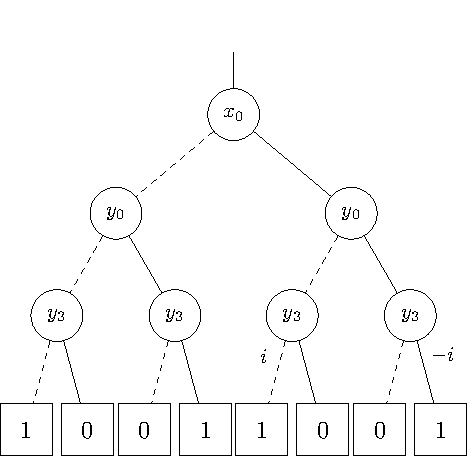
\includegraphics[height=5cm]{Img/tree_norm1.pdf}
        \caption{对图\ref{fig:tdd_ex}的终端节点规范化}
        \label{fig:tdd-norma}
    \end{subfigure}
    \begin{subfigure}[b]{0.4\textwidth}
        \centering
        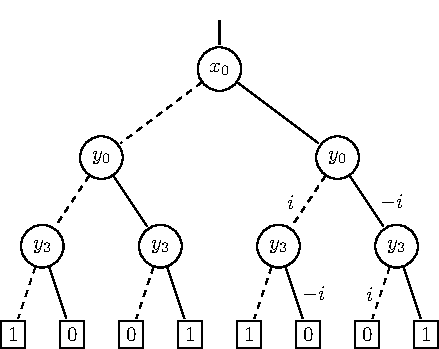
\includegraphics[height=5cm]{Img/tree_norm2.pdf}
        \caption{对图\ref{fig:tdd-norma}的$y_3$节点规范化}
        \label{fig:tdd-normb}
    \end{subfigure}
    \\
    \begin{subfigure}[b]{0.8\textwidth}
        \centering
        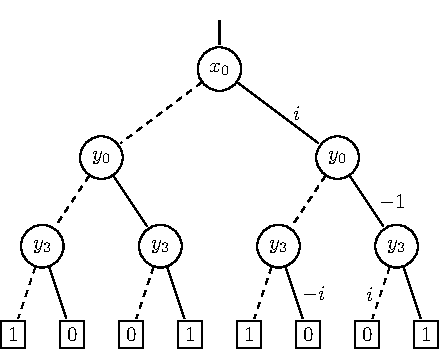
\includegraphics[width=.8\textwidth]{Img/tree_norm3.pdf}
        \caption{对图\ref{fig:tdd_ex}的规范化结果}
        \label{fig:tdd-normc}
    \end{subfigure}
    % \caption{对图\ref{fig:tdd_ex}的规范化过程}
    \label{fig:tdd-norm}
\end{figure}
对于图\ref{fig:tdd_ex}中的TDD。具体规范化过程为:应用第\ref{norm1}步于$i$和$-i$两个终端节点得到图表 \ref{fig:tdd-norma};然后,应用第\ref{norm2}步于右侧两个$y_3$节点,得到图表 \ref{fig:tdd-normb};最后,应用第二条规则于于右侧$y_0$节点。最后可以获得图表 \ref{fig:tdd-normc}。

在完成规范化后,可以进一步简化TDD,使得TDD只包含一个终端节点,同时尽量使用重复出现的张量。具体简化步骤如下:
\begin{myen}
    \item 	合并所有值为1的终端节点。删除所有终端$0$节点,并将它们的入边重定向到唯一的终端节点,并将它们的权重重置为$0$。\label{sympl1}
	\item 将所有权重为$0$的边重定向到终端节点。如果根节点的入边权重为$0$,则终端节点成为新的根,该TDD为空。删除所有从根节点不可达的节点,以及涉及它们的所有边。\label{sympl2}
	\item 如果一个节点v的低边和高边后继相同,并且其低边和高边具有相同的权重w,则删除该节点。如果入边权重$w=0$,则将其传入边重定向到终端节点。否则,将其传入边重定向到其后继节点。\label{sympl3}
	\item 合并两个具有相同索引、相同$0$和$1$后继以及对应边上相同权重的节点。\label{sympl4}
\end{myen}

\begin{figure}[!htbp]
    \centering
    \begin{subfigure}[b]{0.4\textwidth}
        \centering
        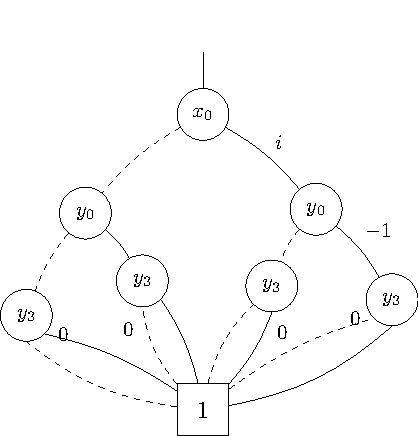
\includegraphics[height = 6cm]{Img/tree_redu1.pdf}
        \caption{对\ref{fig:tdd-normc}中规范TDD的终端节点化简}
        \label{fig:tdd-redu1}
    \end{subfigure}
    \begin{subfigure}[b]{0.4\textwidth}
        \centering
        \includegraphics[height = 6cm]{Img/tree_redu2.pdf}
        \caption{对图\ref{fig:tdd-normc}中规范TDD的简化结果}
        \label{fig:tdd-redu2}
    \end{subfigure}
    \label{fig:tdd-redu}
\end{figure}

对于图\ref{fig:tdd-normc}中规范TDD。具体化简过程为:首先重复第\ref{sympl1} 步,合并所有终端节点,得到图\ref{fig:tdd-redu1};由于没有符合第\ref{sympl2}和第\ref{sympl3}步的节点,因此直接进行第\ref{sympl4}步应用重复第四条规则合并第一个和第三个$y_3$节点,以及第二个和第四个$y_3$节点。最终可以得到\ref{fig:tdd-redu2}所示的简化TDD。

下文中所有的TDD均指化简后的TDD,即reduced tensor decision diagrams。

\subsection{在模型检验中应用TDD}
借助新的数据结构TDD,我们可以更方便的表示量子状态以及量子线路,并计算最终的结果。TDD给出了量子电路的紧凑表示,提供了一种方便的实现张量网络各种操作的方式,这些操作对于模拟量子物理系统非常重要。图表 12展示了一个矩阵和TDD形式,其中TDD中的蓝边表示高边,红边表示低边。可以明显看到TDD的结构更紧凑。
 	 
\begin{figure}[!htbp]
    \begin{subfigure}[c]{0.4\textwidth}
        \centering
        \includegraphics[width=\textwidth]{Img/matrix_of_tdd.pdf}
        \caption{矩阵$P$的矩阵形式}
        \label{fig:mat_P}
    \end{subfigure}
    \begin{subfigure}[c]{0.4\textwidth}
        \centering
        \includegraphics[height=6cm]{Img/tdd_ex.pdf}
        \caption{矩阵$P$的TDD形式}
        \label{fig:tdd_P}
    \end{subfigure}
\end{figure}

TDD特别适用于实现可达性分析和模型检查算法。这是因为基于BDD的模型检查算法中使用的许多优化技术可以推广到收缩量子电路张量网络上\citep{Chaki_2018}。这些为应用TDD解决量子模型检测问题提供了可能的方案。
